\chapter{Implementation}
\label{ch:implementation}

\section{Implementation of the mod}
\subsection{UML diagram of class hierarchy}
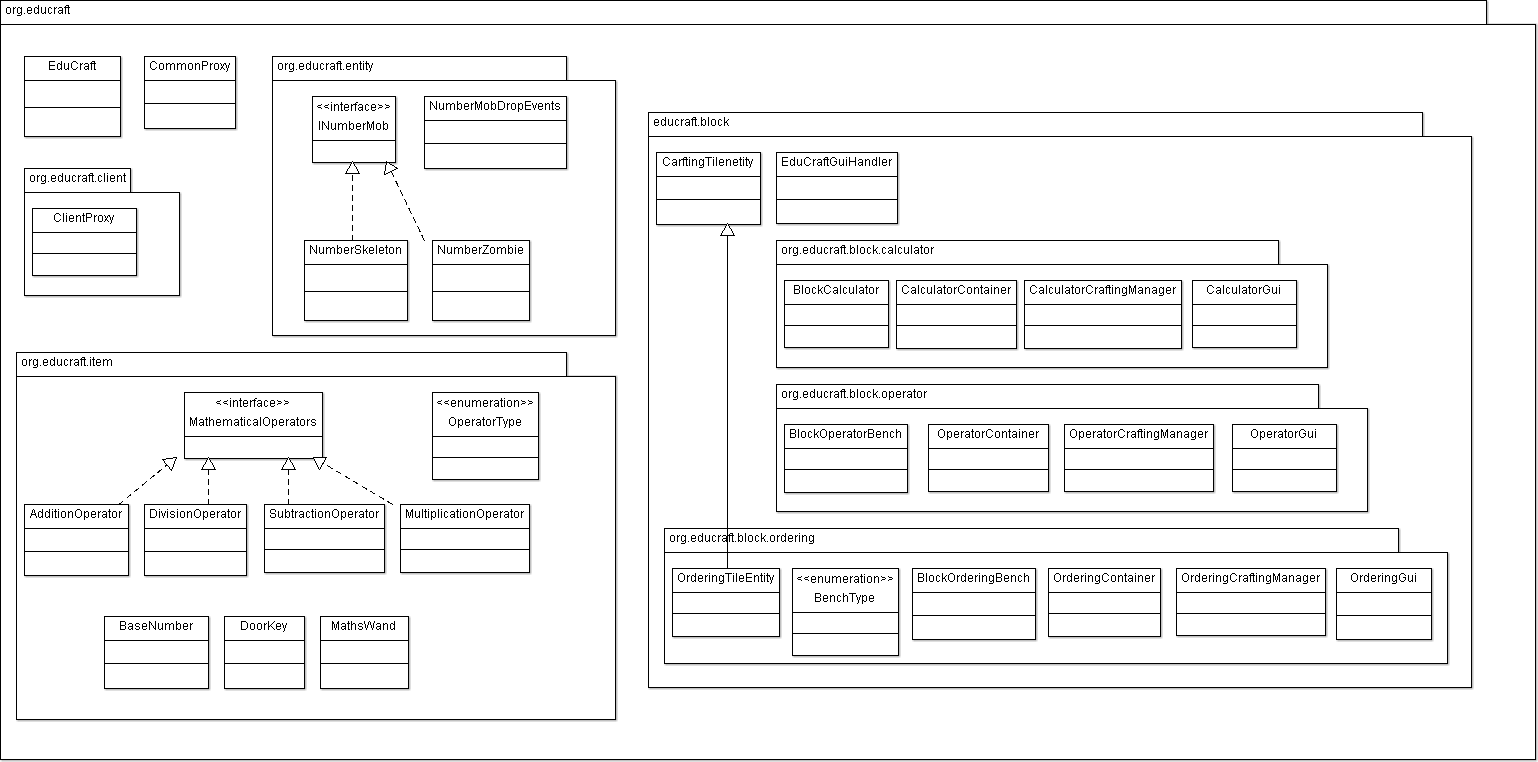
\includegraphics[width=17cm]{ClassDiagram}
\DeclareGraphicsExtensions{.png}
\begin{itemize}
\item \textbf{Base Mod Class}\footnote{``The base class is the class that Forge loads. All the classes in our mod have to be registered through this central location for the mod. It is advised to name this class after the name of the Mod. In our case it is EduCraft''\cite{website:forge-basemods}}\newline
The Base Mod needs to contain the following line:
\begin{lstlisting}
@SidedProxy(clientSide="tutorial.generic.client.ClientProxy",serverSide="tutorial.generic.CommonProxy")
public static CommonProxy proxy;
\end{lstlisting}

\item \textbf{Proxy Classes}\footnote{``Minecraft uses a client and server setup even on single player. The server side does all the maintaining of the world’s state while the client render’s the world. All code runs on both sides unless specified otherwise.\newline
The annotation @SidedProxy is used when we want the server to call the constructor of one class and the client the other. We use the proxy for registering images and hosting our GUI handler.\cite{website:forge-proxy}}
\end{itemize}

\section{Implementation of Constraints}

\section{Implementation of Items}

\section{Implementation of Blocks}
This section covers the most important steps that allowed us to create our own Crafting Tables with custom looks and specific behaviours.\newline\newline
During our initial attempts to create a modified Crafting Table we came across the problem of implementing our Numbers efficiently. We initially thought that we would have to hardcode every single class for each Number item that could be used in the Calculator without having to create separate recipes. This stalled our progress for while, but luckily after a substantial amount of research we found a solution. This workaround allowed us to have one BaseNumber class and every time a new BaseNumber object is created a random metadata is assigned to that specific item. The metadata defines the value, the texture used and the onscreen text displayed for that Number item. After this issue was resolved we were able to proceed with the implementation of the Calculator.\newline\newline
Minecraft distinguishes between two different ways of handling information due to being a multiplayer game, we will refer to these as Server Side and Client Side. The original Crafting Table only opens on the Client Side, which limits the interaction with this object to one player at a time. Initially we started with an implementation that only added custom looks and behaviours to our Crafting Tables. Later on, we recognised the importance of making the Crafting Tables Server Side to allow multiple players to interact with the same block simultaneously. This helped us to create an even more collaborative gaming experience.

\subsection{Chain of method calls during the use of Crafting Table}

\subsection{Extended Block Types}
The Ordering Table has three different types depending on the parity of the input numbers accepted by it. We have created an enum type named BenchType to describe the different types of Ordering Tables. OrderingTileEntity classes are created with an additional field differentiating the specific Ordering Table in the world when the block is created. This attribute will determine the behaviour of the Ordering Tables based on their type.

\subsection{CraftingTileEntity}
We created this class subsequent to our findings relating to the use of the Chest by multiple players simultaneously. We investigated how the Chest worked and found that Tile Entities are used to implement this feature.\newline
Tile Entities are bound to specific coordinates in the world and their fields hold unique values. In the case of the Crafting Table, they hold the inventory of a Block. This allows interaction that can be seen by everyone over the network.\newline
An additional field in our version of the Tile Entities keeps track of the number of players using the Block.\newline
The default constructor is not capable of setting up a crafting matrix (collection of input slots) as the CraftingTileEntity does not have a reference to a container on creation. Our work around was to initialise the CraftingTileEntity as soon as we create a container for a Block.\newline
\begin{lstlisting}
public synchronized CraftingTileEntity initialise(Container container) {
	if (this.container == null) {
		this.container = container;
this.craftMatrix = new InventoryCrafting(this.container, 1, 3);
		this.craftResult = new InventoryCraftResult();
	}
	incrUsers();
	return this;
}
\end{lstlisting}

\subsection{GuiHandler}
This class is essential for handling our custom-made GUIs. It implements the core IGuiHandler interface and has two methods:
\begin{itemize}
\item getServerGuiElement(...)\newline
generates a container, which forms the Server Side of The GUI
\item getClientGuiElement(...)\newline
generates the GUI itself, which is displayed in the Client Side
\end{itemize}

\subsection[Container]{Container\footnote{``The container is what connects the inventories of the player and tileentity to the GUI. The constructor defines the position on-screen and contents of each slot.''\cite{website:forge-container}}}
The following are the changes we made to our extended version of the container to create a custom layout of the slot matrix:
\begin{itemize}

\item in the case of a Client Side only Crafting Table, field in class:
\begin{lstlisting}
public InventoryCrafting craftMatrix = new InventoryCrafting(this, x, y);
\end{lstlisting}

\item in the case of a Server Side Crafting Table, in constructor:
\begin{lstlisting}
this.tileEntity = tileEntity.initialise(this, x, y);
\end{lstlisting}

\let\thefootnote\relax\footnote{x = the number of rows}
\let\thefootnote\relax\footnote{y = the number of columns}

\item in any case, in constructor:
\begin{lstlisting}
// adds output slot to the container
this.addSlotToContainer(new SlotCrafting(inventory.player,	this.craftMatrix, this.craftResult, 0, 124, 35));
			
	// adds input slots to the container
	for (int l = 0; l < x; ++l) {
		for (int i1 = 0; i1 < y; ++i1) {
			this.addSlotToContainer(new Slot(this.craftMatrix, i1 + l * 3, 30 + i1 * 18, 17 + l * 18));
		}
	}
\end{lstlisting}

\let\thefootnote\relax\footnote{x = the number of rows}
\let\thefootnote\relax\footnote{y = the number of columns}
\let\thefootnote\relax\footnote{Please note that in Slot(..., x, y, z) and SlotCrafting(..., x, y, z) the last three arguments passed in are slotIndex, xDisplayPosition and yDisplayPosition in this order. Coordinates are represented in pixels. The default size of a slot is 18x18 pixels.}

\item in the case of a Server Side Crafting Table, in the onContainerClosed() method:	
\begin{lstlisting}
/**
 * Called whenever the container is closed. If no one is using the container
 * any more, then it should drop everything inside it, like a crafting
 * table.
 * 
 * @param player
 *            the player who closed the container
 */
@Override
public void onContainerClosed(EntityPlayer player) {
	super.onContainerClosed(player);
	this.tileEntity.decrUsers();

	if (!this.worldObj.isRemote && !this.tileEntity.isBeingUsed()) {
			for (int i = 0; i < 3; ++i) {
				ItemStack itemstack = this.craftMatrix.getStackInSlotOnClosing(i);
            
				if (itemstack != null) {
					player.dropPlayerItem(itemstack;
				}
			}
	}
}
\end{lstlisting}
\end{itemize}

\subsection{Gui}
This class is responsible for the creation and display of GUIs.
There are two methods within this class. One is responsible for drawing the background and the other one is for drawing the foreground.\newline\newline
\begin{lstlisting}
/**
* Standard prefix for every GUI texture created for the mod.
*/
public static final String GuiTexturePrefix = "educraft" + ":" + "textures/gui/";

private ResourceLocation calculator = new ResourceLocation(EduCraft.GuiTexturePrefix+ "FileName.png");
\end{lstlisting}

\subsection{CraftingManager}
In the Crafting Manager classes for the Calculator and Ordering Bench we simplified the operation of the core version of this class. This was possible as we are not using any Recipes for implementing the logic of how the inputs are checked and the way the output is generated. Both Crafting Tables have only 3 input slots and this allowed us to validate inputs in a simpler manner.\newline\newline
The logic implemented for the Calculator is to have two operands (instance of BaseNumber) in slots 1 and 3 and an operator (instance of MathematicalOperator) in slot 2 of the input matrix. If this condition is not met then there is nothing to generate or else it gets the metadata value (itemDamage) of the operands and the mod internally performs a mathematical operation depending on the type of operator. An output BaseNumber is generated, with the result of the operation stored in the new items metadata. There are a few cases where there is nothing generated even though the operation would be mathematically correct, but our mod does not cover the use of negative numbers, fractions and decimals. We would like to implement these concepts in future versions of the extension.\newline\newline
The Crafting Manager for the Ordering Bench works in a similar way, but it first tests if all the inputs are numbers and then it checks if the order and the parity of the numbers are valid depending on the type of the Ordering Table and finally it generates a coloured key.\newline\newline
We decided to keep the way the core Crafting Manager works for the Operator Bench. This bench has the same behaviour as the core Crafting Table. The only modifications are the visuals and the recipes accepted. We wanted to limit the items that could be crafted by the players in the mod. We achieved this by placing only our own modified versions of the Crafting Tables in our levels. These benches accept only our custom recipes which we defined for the crafting \footnote{``Crafting is the method by which many blocks, tools, and materials are made in Minecraft. In order to craft something, players must move items from their inventory to a crafting grid. A 2×2 crafting grid can be accessed from the player's inventory. A 3×3 grid can be accessed by right-clicking a Crafting Table.''} of the mathematical operators. All these recipes are ShapedRecipes\footnote{``Shaped recipes come in all sizes from 1x1 to 3x3. Strings are used for the recipe shape and values.''\cite{website:forge-shaped}} used in the original version of Minecraft.\newline\newline



